\documentclass[ letterpaper,12pt]{article}

\usepackage[english]{babel}
\usepackage[T1]{fontenc}
\usepackage{a4wide}
\usepackage{graphicx}
%\usepackage{pngfig}

\begin{document}

\title{\textbf{DccNiTghtmare's Documentation 0.0.3}}

\author{
DccNiTghtmare
}

\maketitle

\abstract{This document is the User's manual of the DccNiTghtmare Game.}



\newpage

\tableofcontents

\newpage

\section{Introduction}

Welcome to the user's manual of DccNiTghtmare. Here you'll find all the DccNiTghtmare's computer game related things that you need to know to play DccNiTghtmare on your machine. 

DccNiTghtmare is in {\it public domain}, what means that you can use in any way you want the source code and data of the game: copy it, redistribute it, make a forge of it, modify it, burn it, delete it, blame it, like it, love it, hate it, ... , the only thing that you can't do is to make it your property: it's not an individual property, it's for all property (our way to understand the public domain), it's ideologically for us more free (libre, livre) than the GPL licensing. That's it.

\section{Compiling}

\subsection{Requeriments}

The compilation and execution of DccNiTghtmare requires the follow librarys and hardware:

\subsubsection{Software}
\begin{itemize}
\item{OpenGL  
  \begin{center}
  
\includegraphics{opengl_logo.png}
  \end{center}
}
\item{SDL - Version 1.2.11, www.libsdl.org
\begin{center}
  
\includegraphics{sdl.png}
  \end{center}
}
\item{SDLImage - Version 1.2.5, www.libsdl.org/projects/SDL\_image/}
\item{SDLMixer - Version 1.2.7, www.libsdl.org/projects/SDL\_mixer/}
\item{Cal3D - Version 0.11, http://cal3d.sf.net
\begin{center}
  
\includegraphics{cal3dLogo.png}
  \end{center}
}
\item{LibVorbis - www.vorbis.com}
\end{itemize}

\subsubsection{Hardware}
A video card with 3d aceleration enabled in Linux, compatible with OpenGL (something better than a Geforce 6200 is recommended).

\subsection{Process}

Untar the bzip2 ball with command "tar -xvjf dccnitghtmare-src-003.tar.bz2";\\
Go to the dccnitghtmare folder with "cd dccnitghtmare";\\
Execute the command "make" to make the source code.

\section{Executing}

To Execute DccNiTghtmare, go to the subfolder bin, in the directory dccnitghtmare, and run the program dccnitghtmare.\\
" cd dccnitghtmare/bin "\\
" ./dccnitghtmare "

\subsection{Main Menu}

The main menu window appears on the screen, looking like the bellow {\it figure}. There are five buttons, and the title of the window describes the dccnitghtmare's version.

\begin{center}
  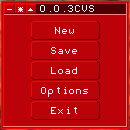
\includegraphics{mainMenuWindow.png}
\\{\bf Figure} - Main Menu Window
\end{center}

The options to choose are:

\begin{itemize}
\item{{\it New Game} - To start a new game with a new character;}
\item{{\it Continue} - To return to the current game ({\it if in game});}
\item{{\it Load} - To load an existent game; {\bf Not yet implemented!}}
\item{{\it Save} - To save the current game ({\it if in game}); {\bf Not yet implemented!}}
\item{{\it Options} - To manipulate the game options;}
\item{{\it Exit} - To exit the game;}
\end{itemize}

\subsection{Options}

\begin{center}
  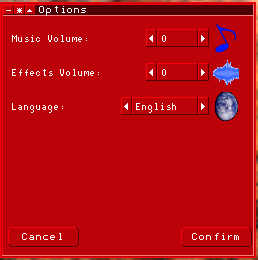
\includegraphics{optionsWindow.png}
\\{\bf Figure} - Options Window
\end{center}

In the options window you can change music and sound effects volume ( =0 means no sound or no music) and change the main language of the game. For now we offer full support to Portuguese and English languages and incomplete support to French and Spanish.

\section{Creating Character}

Like DccNiTghtmare is a rpg D\&D friendly game, the player have to create a character to play, with unique stats. All things that a player character can be are describeded in the DccNiTghtmare Player's Book, avaible at http://dccnitghtmare.sf.net .

All rpg rules are D\&D like, so if you played the D\&D somewhere you'll easy understand all character's things here.

\subsection{Race}

{\bf WINDOW NOT YET IMPLEMENTED}

\subsection{Aligment \& Gender}

{\bf WINDOW NOT YET IMPLEMENTED}

\subsection{Attributes}

{\bf WINDOW NOT YET IMPLEMENTED}

\subsection{Class}

{\bf WINDOW NOT YET IMPLEMENTED}

\subsection{Skills}

\begin{center}
  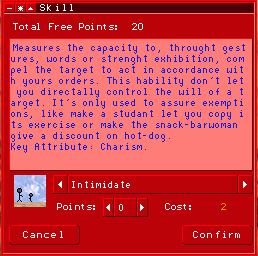
\includegraphics{skillWindow.png}
\\{\bf Figure} - Skills Window
\end{center}

In the skills window, you can redistribute all your avaible points to the skills you want. The cost of each skill means how many free points you'll need to increase one point in the skill.

The number of avaible skill points vary based on character's class and race, and also, level.

\subsection{Feats}

{\bf WINDOW NOT YET IMPLEMENTED}

\section{In-Game}

The main game window is composed by 2 basic windows, the visualization of the world and the player's portrait. Bellow we'll describe them.

\begin{center}
  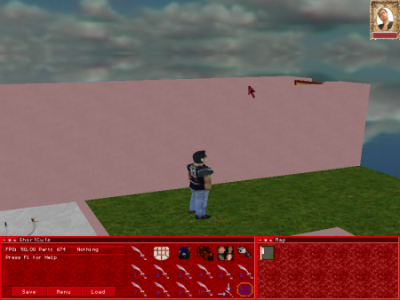
\includegraphics{mainGame.png}
\\{\bf Figure} - Main Game Window
\end{center}

\subsection{ShortCuts Window}

\begin{center}
  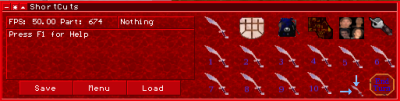
\includegraphics{shortcutsWindow.png}
\\{\bf Figure} - ShortCuts Window
\end{center}

The ShortCuts window is used to give the user many informations of things current occurring on game and, also, to take from them some basic actions.

The window is composed, on the left corner, from 3 text boxes: the upper left one, show the current FPS of the game (limited to 50) and actual number of particles in map; the upper right one, describe the name of the object or reactor pointed by user's mouse; the last one show informations about the fight, if in fight mode.

Also, in the left corner, three shortcut buttons exists. One to load an saved game ({\it the load function is not yet implemented}), other to go to the main game menu, and the last to save the game ({\it the save function is not yet implemented}).

On the right corner, there are shortcuts 18 buttons. From left to right they are, on the first row: Button to enter the attack mode (with surprise attack to the player character), to enter the defend mode, to open the player's inventory, to open the map window, to open the party window, to view the player character's informations. On the second row, the first six shortcuts to assigned attacks. On the third row, the last four shortcuts to assigned attacks, the button to open the assign attacks window and the button to end the player character's turn.

This window can be opened by the keyboard 'n' key.

\subsection{Map Window}

\begin{center}
  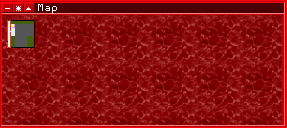
\includegraphics{mapWindow.png}
\\{\bf Figure} - Map Window
\end{center}

The map window represent the actual world map that is open. Also, the yellow square represents the current player character's position on the map. 

This window can be opened by the keyboard 'm' key, or by the map button on ShortCuts window.

\subsection{Character's Portrait}

\begin{center}
  
\includegraphics{portrait.png}
\\{\bf Figure} - Character's Portrait
\end{center}

The character's portrait represents the active player character, and his health status. There are a health bar (in red), showing how much of the total life points actual left.

\subsection{Keyboard Commands}

\begin{tabular}{|c|c|}
\hline
F1 & Open quick help screen\\
\hline
Esc & Go To Main Menu\\
\hline
0-9 & Shortcut to assigned attacks\\
\hline
a & Turn Left\\
d & Turn Right\\
w & Step Forward\\
s & Step Backward\\
q & Step Left\\
e & Step Right\\
\hline
Left Arrow & Turn Camera Left\\
Right Arrow & Turn Camera Right\\
Up Arrow & Increases Zoom\\
Down Arrow & Decreases Zoom\\
Home & Maximize Zoom\\
End & Minimize Zoom\\
PageUp & Move Camera Up\\
PageDown & Move Camera Down\\
Insert & Move Camera to Top\\
Delete & Move Camera to Floor\\
\hline
\end{tabular}

\subsection{Mouse Commands}

\begin{tabular}{|c|c|}
\hline
 
\includegraphics{Get.png} & Get, if posible, an object\\
\hline
 
\includegraphics{Door.png} & Open, if possible, a door\\
\hline
 
\includegraphics{MapTravel.png} & Travel to another map\\
\hline
 
\includegraphics{Walk.png} & Walk with the character to some map point\\
\hline
 
\includegraphics{talk.png} & In normal mode, talk to a character\\
\hline
 
\includegraphics{Attack.png} & If in attack mode, attack a character\\
\hline
\end{tabular}

\subsection{Fighting}

The fighting mode is, in somethings, distict than the normal mode of the game. Here your movimentation is limited and the action is taked in turns.

The game goes to fight mode each time when there are enemies in renge area (and they want to attack your character) or you want to attack any NPC in the area.

\subsubsection{Initing a Fight}

When you want to init by yourself the fight mode, you can use the button of fight in the ShortCuts Window. By done it, you enter in the fight mode, in your active character's turn (called surprise attack turn) where functions like any other normal turn. If at the end of this turn you've not attacked, the game exits the attack mode. Otherwise, continue the fight in the  correspondent initiative values orderf.

\subsubsection{Player Character's Turn}

\begin{center}
  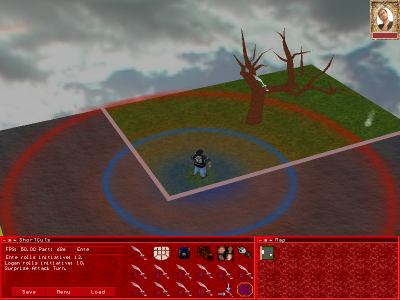
\includegraphics{fightMode.png}
\\{\bf Figure} - Fight Mode
\end{center}

When is player character's turn, like D\&D, the character can take a standart action and a move action, in any order, two move actions or a full round action. The area that the character can walk with one move action is represented in the blue circle; the two move actions is represented in the red circle.

The player choose the actions to be made on the turn, doing all of them and, when done with it, end the turn.

\subsubsection{End Turn}

When you done all things that you want (and that you can) in your turn, you can pass the fight to next character's turn. You can do it by clicking in the ShortCuts Window button of End Turn.

\subsection{Talking}

To talk to a NPC you need to be on normal game mode, put your mouse cursor in the target NPC, showing the talk mouse cursor 
\includegraphics{talk.png}, and press the left mouse button.

The talk window will open, showing the things npc talked and the options your character can talk to him. You need do be in range to can talk, with your character get out of range, the conversation will be stop, like you abandoned it.

{\bf NOT YET IMPLEMENTED!}

\subsection{Inventory}

{\bf NOT YET IMPLEMENTED!}

\subsection{Sugestions and Help}

We are an open group, if you have some sugestions to to DccNiTghtmare or want to help the development of the game in some manners, just contact us at sourceforge.

\end{document}

